در این بخش صرفا خروجی کد و اسکرین‌شات‌های WireShark را قرار می‌دهیم. توضیحات کامل‌تر کد و نحوه پیاده‌سازی، داخل فایل REAMDE هر کد موجود است. در حل این سوال ناچارا از مدل‌های زبانی بزرگ استفاده شده است.

\subsectionaddtolist{آ}

ابتدا به صورت عادی پیام‌ها را ارسال می‌کنیم و می‌بینیم که به صورت Fragmented برای سرور ارسال شده است و دارای TTL درست است. 

\begin{center}
	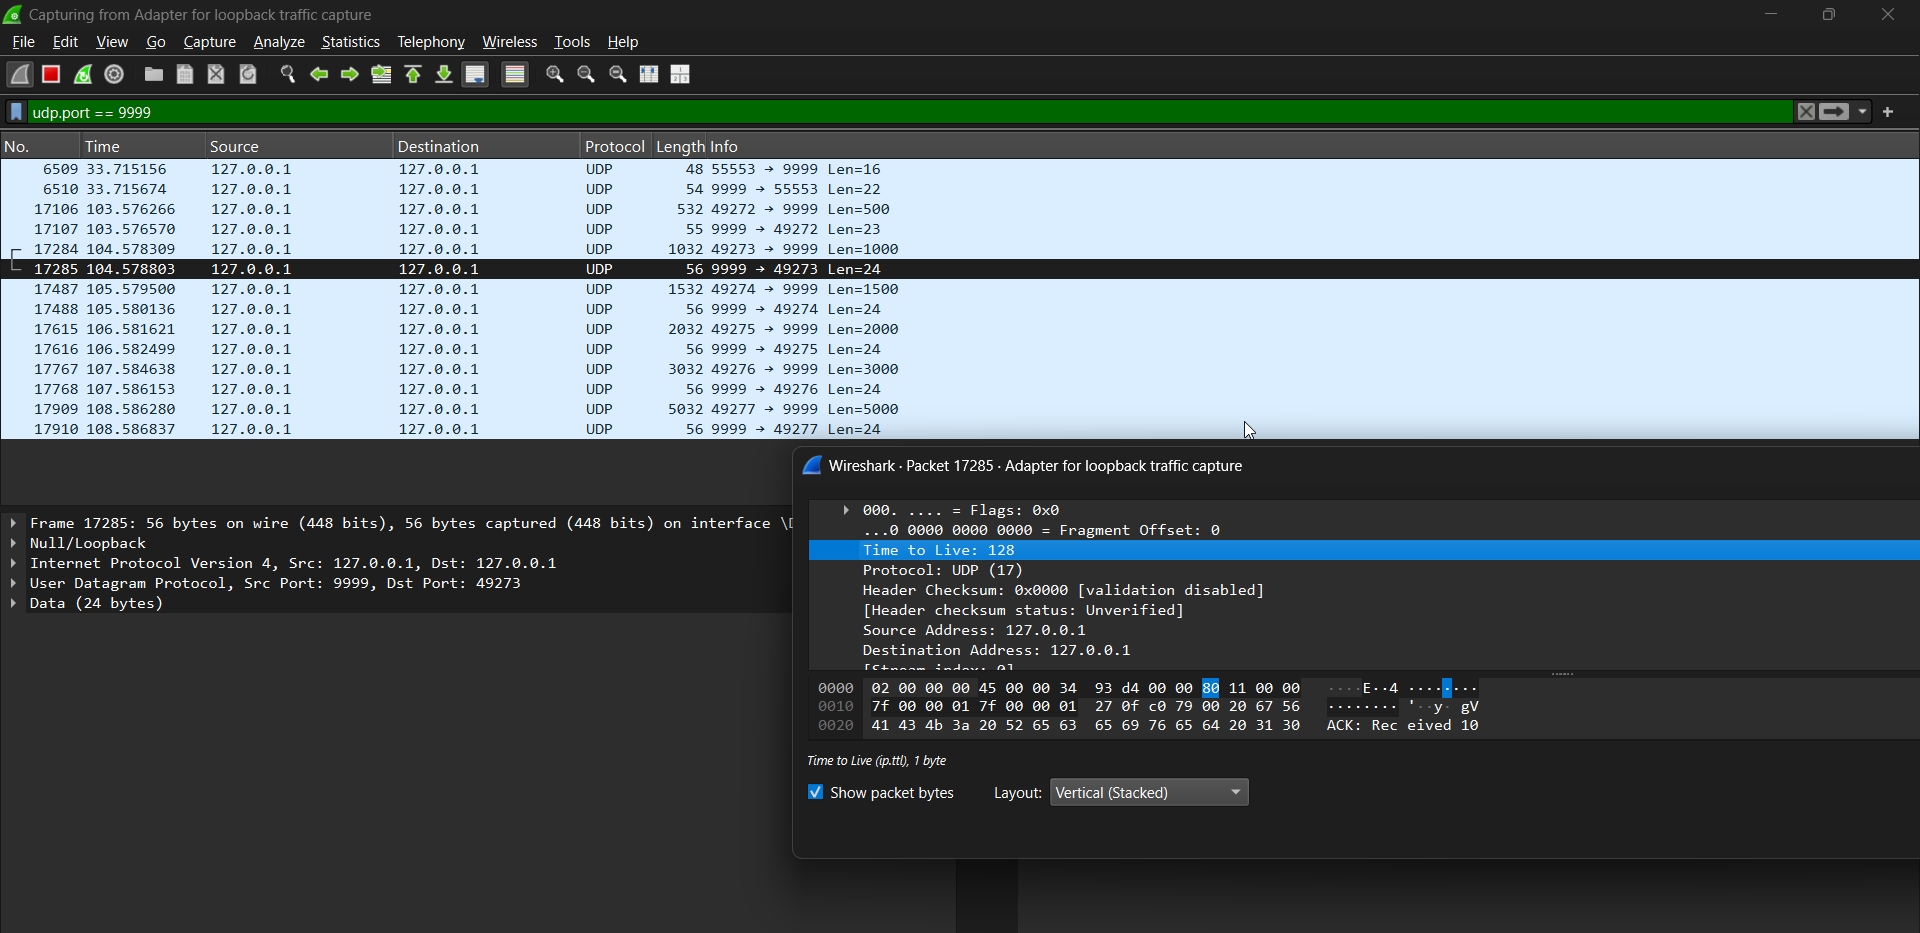
\includegraphics[width=0.8\linewidth]{screenshot001}
\end{center}
	

همچنین پیام‌ها در سرور به درستی تحویل داده شده‌اند:

\begin{center}
	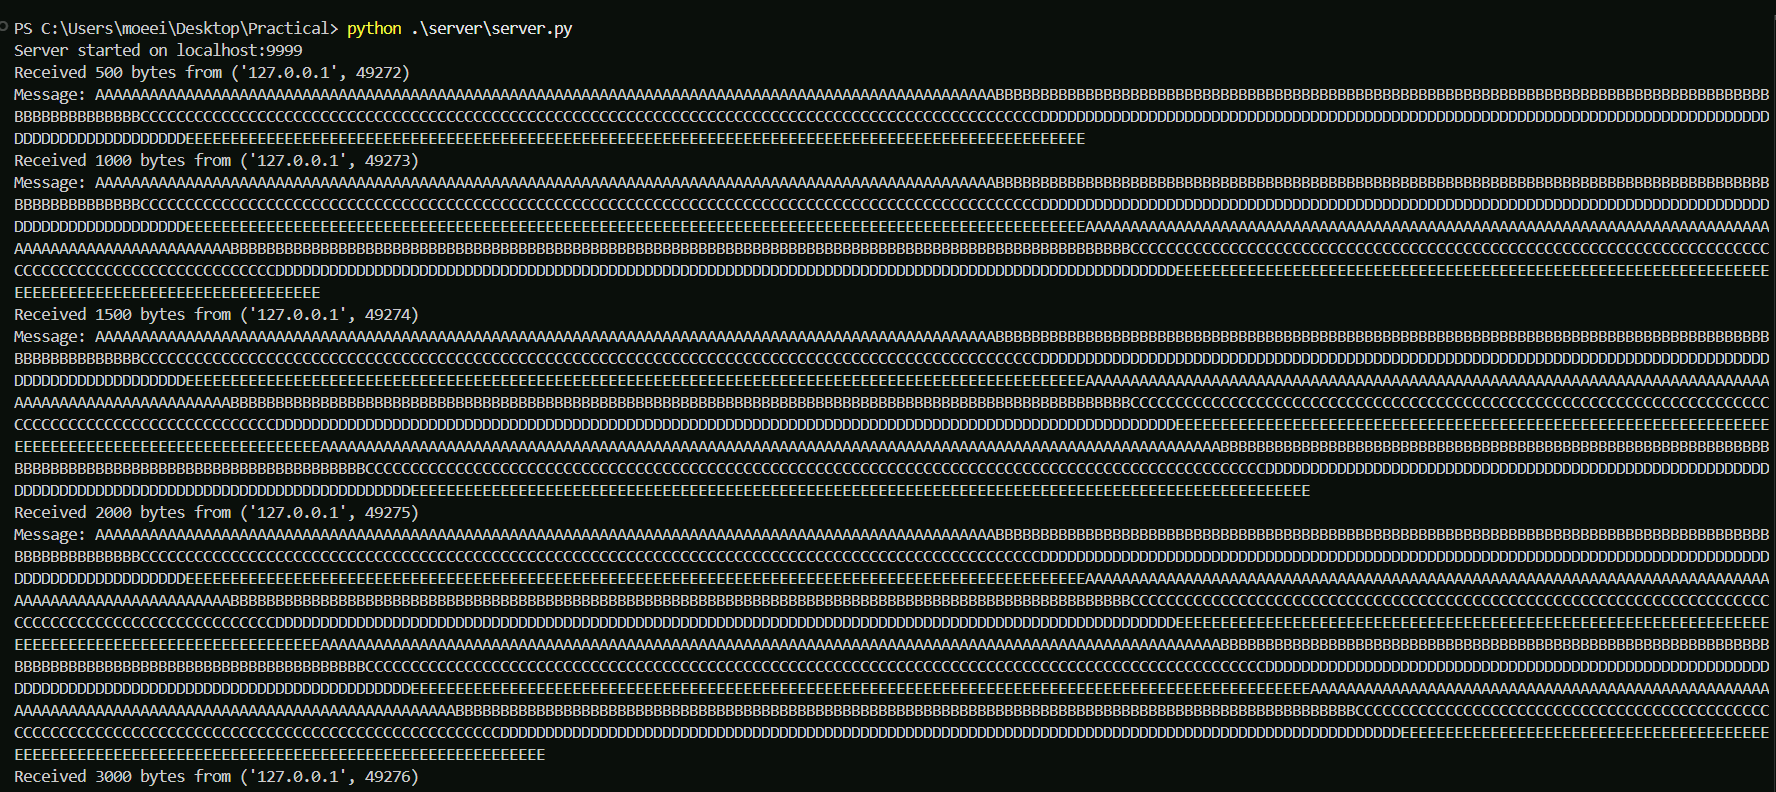
\includegraphics[width=0.8\linewidth]{screenshot002}
\end{center}

\pagebreak


\subsectionaddtolist{ب}

در این بخش قرار است مقدار TTL را خودمان تنظیم کنیم و مقدار ثابت 1 را برای هر فرگمنت قرار دهیم تا توسط فایروال سرور قابل ردیابی نباشد.

کد کلاینت را ران می‌کنیم. همانطور که در تصویر می‌بینید این کد دارای حالت‌های مختلف برای تست کردن است که توضیحات آن در فایل README موجود است.
\begin{center}
	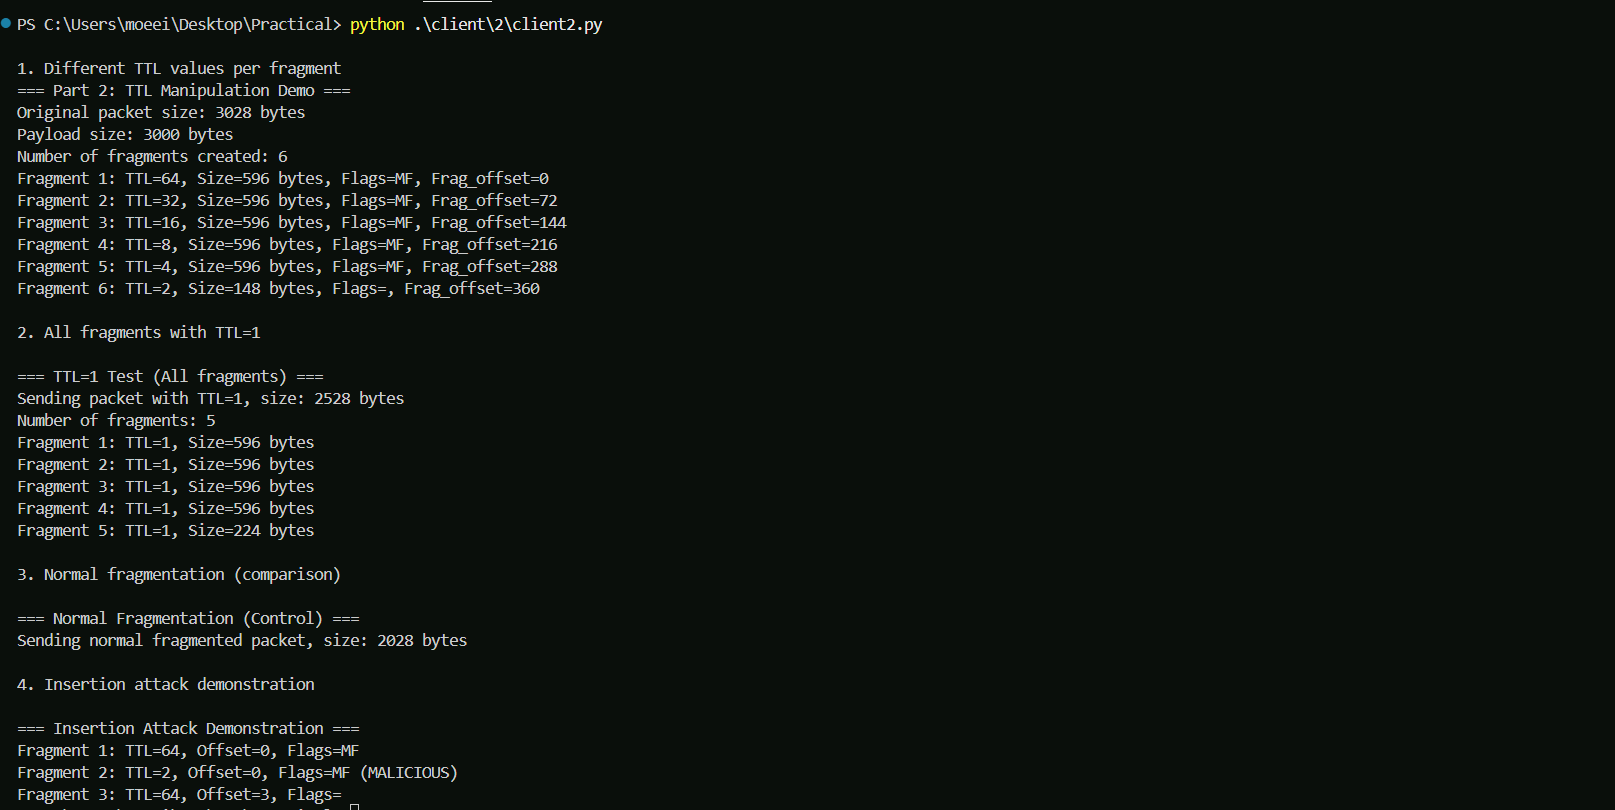
\includegraphics[width=0.8\linewidth]{screenshot003}
\end{center}

تاییدیه دریافت پیام در سرور:

\begin{center}
	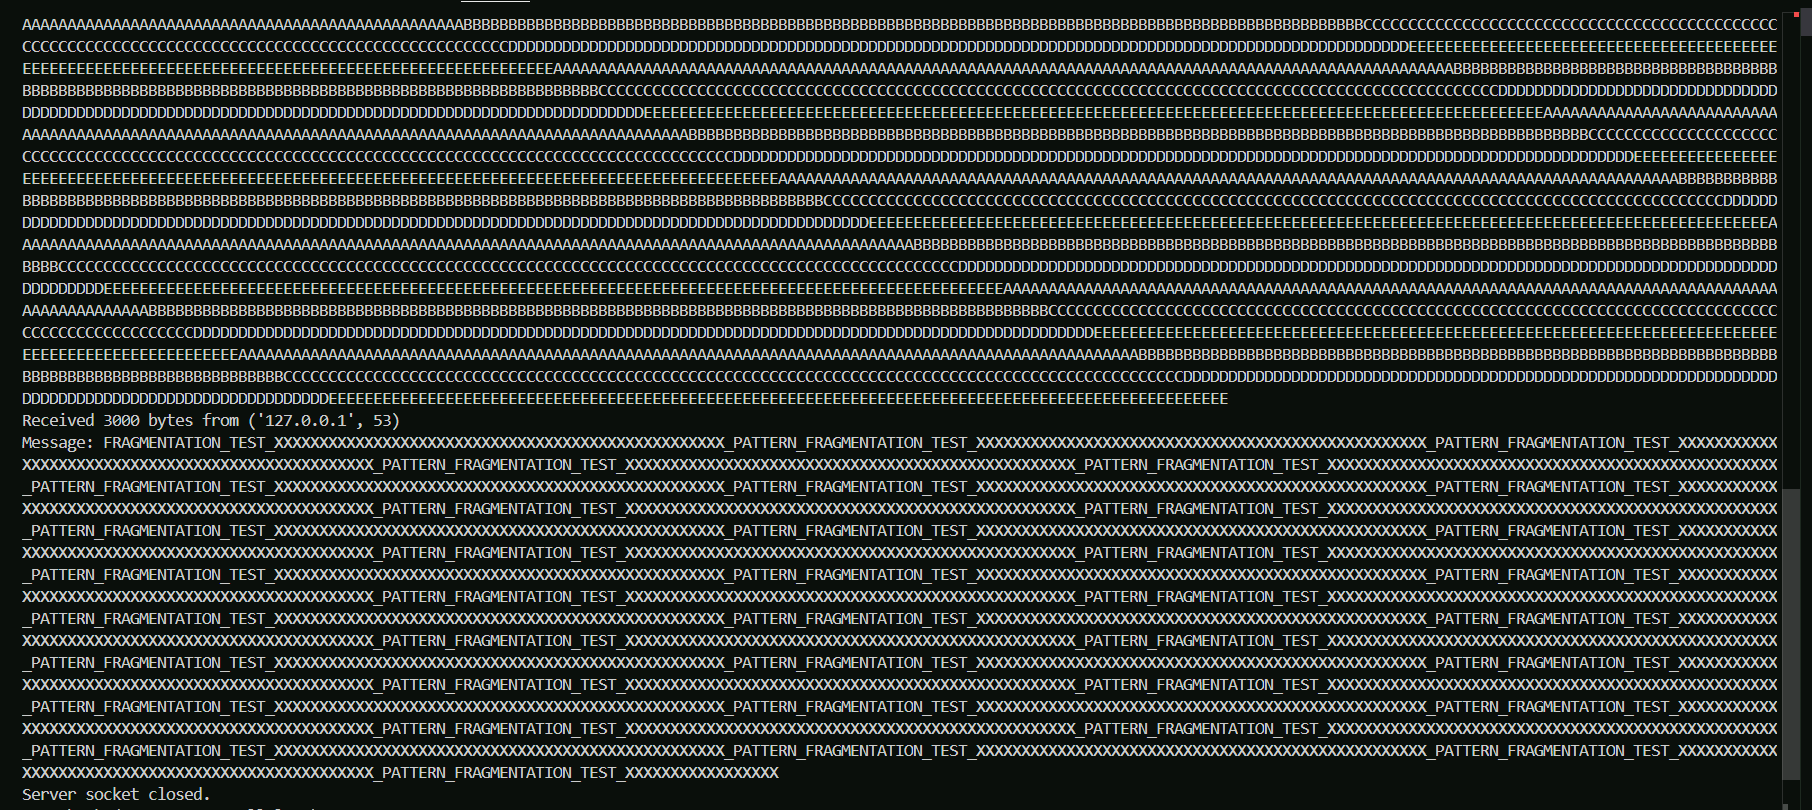
\includegraphics[width=0.8\linewidth]{screenshot004}
\end{center}


در Wireshark به دلیل اینکه TTL برابر با 1 ست شده، این بسته را قرمز نشان داده است. اما در عکس ترمینال سرور مشخص است که بست به درستی به دست سرور رسیده است:

\begin{center}
	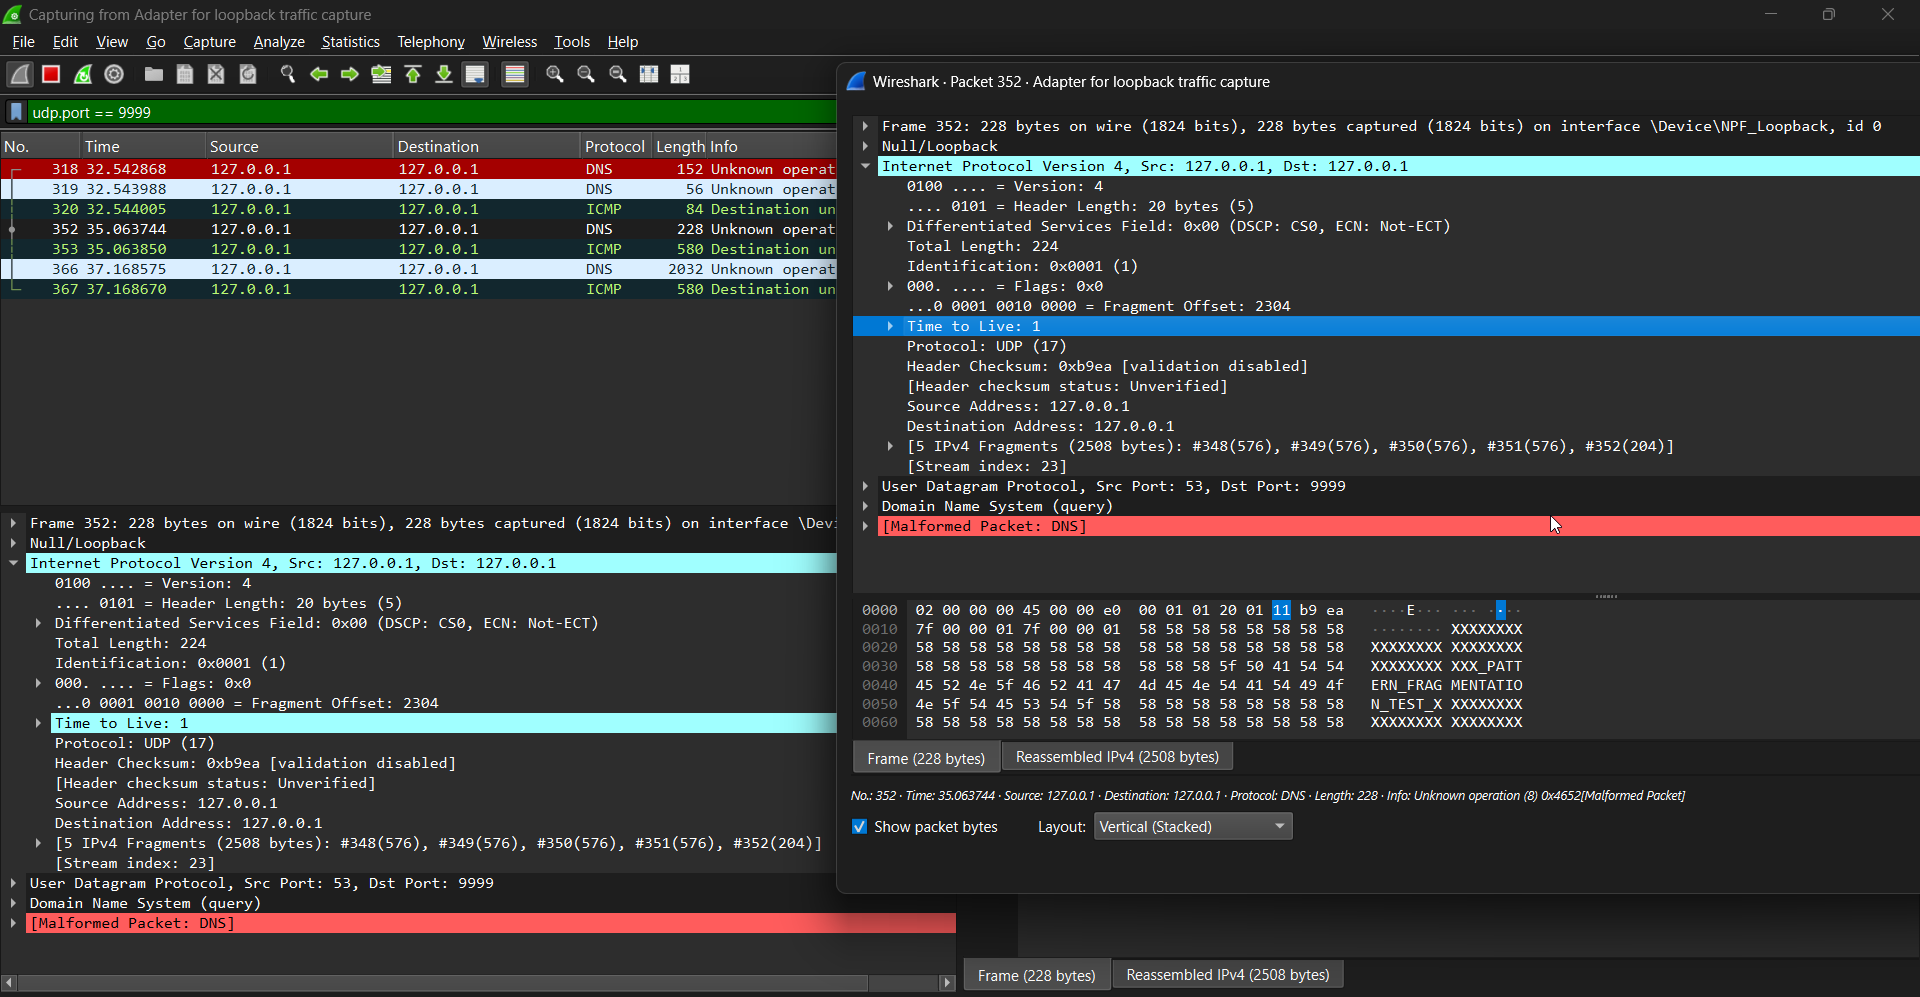
\includegraphics[width=1\linewidth]{screenshot005}
\end{center}
